\documentclass[10pt,a4paper]{article}

\usepackage[spanish,activeacute,es-tabla]{babel}
\usepackage[utf8]{inputenc}
\usepackage{ifthen}
\usepackage{listings}
\usepackage{dsfont}
\usepackage{subcaption}
\usepackage{amsmath}
\usepackage[strict]{changepage}
\usepackage[top=1cm,bottom=2cm,left=1cm,right=1cm]{geometry}%
\usepackage{color}%
\newcommand{\tocarEspacios}{%
	\addtolength{\leftskip}{3em}%
	\setlength{\parindent}{0em}%
}

% Especificacion de procs

\newcommand{\In}{\textsf{in }}
\newcommand{\Out}{\textsf{out }}
\newcommand{\Inout}{\textsf{inout }}

\newcommand{\encabezadoDeProc}[4]{%
	% Ponemos la palabrita problema en tt
	%  \noindent%
	{\normalfont\bfseries\ttfamily proc}%
	% Ponemos el nombre del problema
	\ %
	{\normalfont\ttfamily #2}%
	\
	% Ponemos los parametros
	(#3)%
	\ifthenelse{\equal{#4}{}}{}{%
		% Por ultimo, va el tipo del resultado
		\ : #4}
}

\newenvironment{proc}[4][res]{%
	
	% El parametro 1 (opcional) es el nombre del resultado
	% El parametro 2 es el nombre del problema
	% El parametro 3 son los parametros
	% El parametro 4 es el tipo del resultado
	% Preambulo del ambiente problema
	% Tenemos que definir los comandos requiere, asegura, modifica y aux
	\newcommand{\requiere}[2][]{%
		{\normalfont\bfseries\ttfamily requiere}%
		\ifthenelse{\equal{##1}{}}{}{\ {\normalfont\ttfamily ##1} :}\ %
		\{\ensuremath{##2}\}%
		{\normalfont\bfseries\,\par}%
	}
	\newcommand{\asegura}[2][]{%
		{\normalfont\bfseries\ttfamily asegura}%
		\ifthenelse{\equal{##1}{}}{}{\ {\normalfont\ttfamily ##1} :}\
		\{\ensuremath{##2}\}%
		{\normalfont\bfseries\,\par}%
	}
	\renewcommand{\aux}[4]{%
		{\normalfont\bfseries\ttfamily aux\ }%
		{\normalfont\ttfamily ##1}%
		\ifthenelse{\equal{##2}{}}{}{\ (##2)}\ : ##3\, = \ensuremath{##4}%
		{\normalfont\bfseries\,;\par}%
	}
	\renewcommand{\pred}[3]{%
		{\normalfont\bfseries\ttfamily pred }%
		{\normalfont\ttfamily ##1}%
		\ifthenelse{\equal{##2}{}}{}{\ (##2) }%
		\{%
		\begin{adjustwidth}{+5em}{}
			\ensuremath{##3}
		\end{adjustwidth}
		\}%
		{\normalfont\bfseries\,\par}%
	}
	
	\newcommand{\res}{#1}
	\vspace{1ex}
	\noindent
	\encabezadoDeProc{#1}{#2}{#3}{#4}
	% Abrimos la llave
	\par%
	\tocarEspacios
}
{
	% Cerramos la llave
	\vspace{1ex}
}

\newcommand{\aux}[4]{%
	{\normalfont\bfseries\ttfamily\noindent aux\ }%
	{\normalfont\ttfamily #1}%
	\ifthenelse{\equal{#2}{}}{}{\ (#2)}\ : #3\, = \ensuremath{#4}%
	{\normalfont\bfseries\,;\par}%
}

\newcommand{\pred}[3]{%
	{\normalfont\bfseries\ttfamily\noindent pred }%
	{\normalfont\ttfamily #1}%
	\ifthenelse{\equal{#2}{}}{}{\ (#2) }%
	\{%
	\begin{adjustwidth}{+2em}{}
		\ensuremath{#3}
	\end{adjustwidth}
	\}%
	{\normalfont\bfseries\,\par}%
}

% Tipos

\newcommand{\nat}{\ensuremath{\mathds{N}}}
\newcommand{\ent}{\ensuremath{\mathds{Z}}}
\newcommand{\float}{\ensuremath{\mathds{R}}}
\newcommand{\bool}{\ensuremath{\mathsf{Bool}}}
\newcommand{\cha}{\ensuremath{\mathsf{Char}}}
\newcommand{\str}{\ensuremath{\mathsf{String}}}

% Logica

\newcommand{\True}{\ensuremath{\mathrm{true}}}
\newcommand{\False}{\ensuremath{\mathrm{false}}}
\newcommand{\Then}{\ensuremath{\rightarrow}}
\newcommand{\Iff}{\ensuremath{\leftrightarrow}}
\newcommand{\implica}{\ensuremath{\longrightarrow}}
\newcommand{\IfThenElse}[3]{\ensuremath{\mathsf{if}\ #1\ \mathsf{then}\ #2\ \mathsf{else}\ #3\ \mathsf{fi}}}
\newcommand{\yLuego}{\land _L}
\newcommand{\oLuego}{\lor _L}
\newcommand{\implicaLuego}{\implica _L}

\newcommand{\cuantificador}[5]{%
	\ensuremath{(#2 #3: #4)\ (%
		\ifthenelse{\equal{#1}{unalinea}}{
			#5
		}{
			$ % exiting math mode
			\begin{adjustwidth}{+2em}{}
				$#5$%
			\end{adjustwidth}%
			$ % entering math mode
		}
		)}
}

\newcommand{\existe}[4][]{%
	\cuantificador{#1}{\exists}{#2}{#3}{#4}
}
\newcommand{\paraTodo}[4][]{%
	\cuantificador{#1}{\forall}{#2}{#3}{#4}
}

%listas

\newcommand{\TLista}[1]{\ensuremath{seq \langle #1\rangle}}
\newcommand{\lvacia}{\ensuremath{[\ ]}}
\newcommand{\lv}{\ensuremath{[\ ]}}
\newcommand{\longitud}[1]{\ensuremath{|#1|}}
\newcommand{\cons}[1]{\ensuremath{\mathsf{addFirst}}(#1)}
\newcommand{\indice}[1]{\ensuremath{\mathsf{indice}}(#1)}
\newcommand{\conc}[1]{\ensuremath{\mathsf{concat}}(#1)}
\newcommand{\cab}[1]{\ensuremath{\mathsf{head}}(#1)}
\newcommand{\cola}[1]{\ensuremath{\mathsf{tail}}(#1)}
\newcommand{\sub}[1]{\ensuremath{\mathsf{subseq}}(#1)}
\newcommand{\en}[1]{\ensuremath{\mathsf{en}}(#1)}
\newcommand{\cuenta}[2]{\mathsf{cuenta}\ensuremath{(#1, #2)}}
\newcommand{\suma}[1]{\mathsf{suma}(#1)}
\newcommand{\twodots}{\ensuremath{\mathrm{..}}}
\newcommand{\masmas}{\ensuremath{++}}
\newcommand{\matriz}[1]{\TLista{\TLista{#1}}}
\newcommand{\seqchar}{\TLista{\cha}}

\renewcommand{\lstlistingname}{Código}
\lstset{% general command to set parameter(s)
	language=Java,
	morekeywords={endif, endwhile, skip},
	basewidth={0.47em,0.40em},
	columns=fixed, fontadjust, resetmargins, xrightmargin=5pt, xleftmargin=15pt,
	flexiblecolumns=false, tabsize=4, breaklines, breakatwhitespace=false, extendedchars=true,
	numbers=left, numberstyle=\tiny, stepnumber=1, numbersep=9pt,
	frame=l, framesep=3pt,
	captionpos=b,
}

\usepackage{caratula} % Version modificada para usar las macros de algo1 de ~> https://github.com/bcardiff/dc-tex


\titulo{Trabajo práctico 1}
\subtitulo{Especificación y WP}

\fecha{21/4/2024}

\materia{AED}
\grupo{Grupo IATOGYSWWBKAFJVCRWKR}

\integrante{Calo, Agustín}{390/23}{caloagustin4@gmail.com}
\integrante{Seri, Rafael Nicolás}{002/01}{email2@dominio.com}
\integrante{Pintos Oliveira, Sol Maria Marcela}{428/23}{solpintosoliveira@gmail.com}
\integrante{Paez Torrico, Santiago}{713/23}{santiagopaez122@gmail.com}
% Pongan cuantos integrantes quieran

% Declaramos donde van a estar las figuras
% No es obligatorio, pero suele ser comodo
\graphicspath{{../static/}}

\begin{document}









\maketitle
\section{Especificación}



\subsection{redistribucionDeLosFrutos}
\begin{proc}{redistribucionDeLosFrutos}{\In recursos: \TLista{\float}, \In cooperan : \TLista{\bool}} {\TLista{\float}}
	\requiere {-}
	\asegura{-}
\end{proc}


\subsection{trayectoriaDeLosFrutosIndividualesALargoPlazo}
\begin{proc}{trayectoriaDeLosFrutosIndividualesALargoPlazo}{\Inout trayectorias: \TLista{\TLista{\float}}, \In cooperan: \TLista{\bool}, \In apuestas: \TLista{\TLista{\float}}, \In pagos: \TLista{\TLista{\float}}, \In eventos: \TLista{\TLista{\float}}} {}
	\requiere {-}
	\asegura{-}
\end{proc}


\subsection{trayectoriaExtrañaEscalera}
\begin{proc}{trayectoriaExtrañaEscalera}{\In trayectorias: \TLista{\float}} {\bool}
	\requiere {-}
	\asegura{-}
\end{proc}


\subsection{individuoDecideSiCooperarONo}
\begin{proc}{individuoDecideSiCooperarONo}{\In individuo: \nat, \In recursos: \TLista{\float}, \Inout cooperan: \TLista{\bool}, \In apuestas: \TLista{\TLista{\float}}, \In pagos: \TLista{\TLista{\float}}, \In eventos: \TLista{\TLista{\nat}}} {}
	\requiere {-}
	\asegura{-}
\end{proc}


\subsection{individuoActualizaApuesta}
\begin{proc}{individuoActualizaApuesta}{\In individuo: \nat, \In recursos: \TLista{\float}, \In cooperan: \TLista{\bool}, \Inout apuestas: \TLista{\TLista{\bool}}, \In pagos: \TLista{\TLista{\float}}, \In eventos: \TLista{\TLista{\nat}}} {}
	\requiere {-}
	\asegura{-}
\end{proc}







\section{Demostraciones de correctitud}

Demostrar que la siguiente especificación es correcta respecto de su implementación.

La función \textbf{frutoDelTrabajoPuramenteIndividual} calcula, para el ejemplo de apuestas al juego de cara o seca, cuánto se ganaría si se juega completamente solo. Se contempla que el evento True es cuando sale cara.

\begin{proc}{frutoDelTrabajoPuramenteIndividual}{\In recurso: \float, \In apuesta: \ensuremath{\langle s: \float, c: \float \rangle}, \In pago: \ensuremath{\langle s: \float, c: \float \rangle}, \In eventos: \TLista {\bool}, \Out res: \float } {}
	\requiere {apuesta_c + apuesta_s = 1 \land pago_c > 0 \land pago_s > 0 \land apuesta_c > 0 \land apuesta_s > 0 \land recurso > 0}
	\asegura{res = recurso(apuesta_c pago_c)^{\#apariciones(eventos,T)} (apuesta_s pago_s)^{\#apariciones(eventos,F )}}
\end{proc}

Donde \#apariciones(eventos, T) es el auxiliar utilizado en la teórica, y \#(eventos, T) es su abreviación.
\begin{lstlisting}
	res := recursos
	i := 0
	while (i < |eventos|) do
		if eventos[i] then
			res := (res * apuesta.c) * pago.c
		else
			res := (res * apuesta.s) * pago.s
		endif
		i := i + 1
	endwhile
	\end{lstlisting}




























Lo principal: las fórmulas. Se puede poner en una linea, como $x_i = x_{i-1} + x_{i-2}$, o ponerse más grande:

\begin{equation}
	\sum\limits_{i=0}^{n} i
	\label{eq:1}
\end{equation}

Y se pueden citar ecuaciones con \verb|\eqref{nombreDeEq}|: \eqref{eq:1}

Ejemplo de itemizado:

\begin{itemize}
	\item Item 1
	\item Item 2
	\item Item 3
\end{itemize}

Ejemplo de enumerado con menor distancia entre items:

\begin{enumerate} \setlength\itemsep{0cm}
	\item Item 1
	\item Item 2
	\item Item 3
\end{enumerate}

Podemos escribir mucho texto. Mucho texto. Mucho texto. Mucho texto. Mucho texto. Mucho texto. Mucho texto. Mucho texto. Mucho texto. Mucho texto. Mucho texto.

Otro párrafo. Otro párrafo. Otro párrafo. Otro párrafo. Otro párrafo. Otro párrafo. Otro párrafo. Otro párrafo. Otro párrafo. Otro párrafo. Otro párrafo. Otro párrafo. Otro párrafo.

\vspace{0.3cm}

Le agregamos una separación entre párrafos. Le agregamos una separación entre párrafos. Le agregamos una separación entre párrafos. Le agregamos una separación entre párrafos. Le agregamos una separación entre párrafos.

\vspace{0.3cm}

La tabla \ref{tab:ejemplo} es un ejemplo de cómo se hace una tabla.

\begin{table}[h!]
	\centering
	\begin{tabular}{||l c c r||} 
		\hline
		Col1 & Col2 & Col2 & Col3 \\ [0.5ex] 
		\hline\hline
		1 & 6 & 87837 & 787 \\ 
		2 & 7 & 78 & 5415 \\
		3 & 545 & 778 & 7507 \\
		4 & 545 & 18744 & 7560 \\
		5 & 88 & 788 & 6344 \\
		\hline
	\end{tabular}
	\caption{Ejemplo de tabla}
	\label{tab:ejemplo}
\end{table}


La figura \ref{fig:subfigs} es un ejemplo de cómo se agrega una imagen.

\begin{figure}[ht]
	\centering
	
\includegraphics[width=0.6\textwidth]{logo_dc.jpg}
	\caption{Ejemplo de figura}
	\label{fig:ejemplo}
\end{figure}

\begin{figure}[ht!]
	\begin{subfigure}{0.5\textwidth}
		
\includegraphics[width=0.9\linewidth]{LaTeX-project} 
		\caption{Logo de LaTeX}
		\label{fig:subfig1}
	\end{subfigure}
	\begin{subfigure}{0.5\textwidth}
		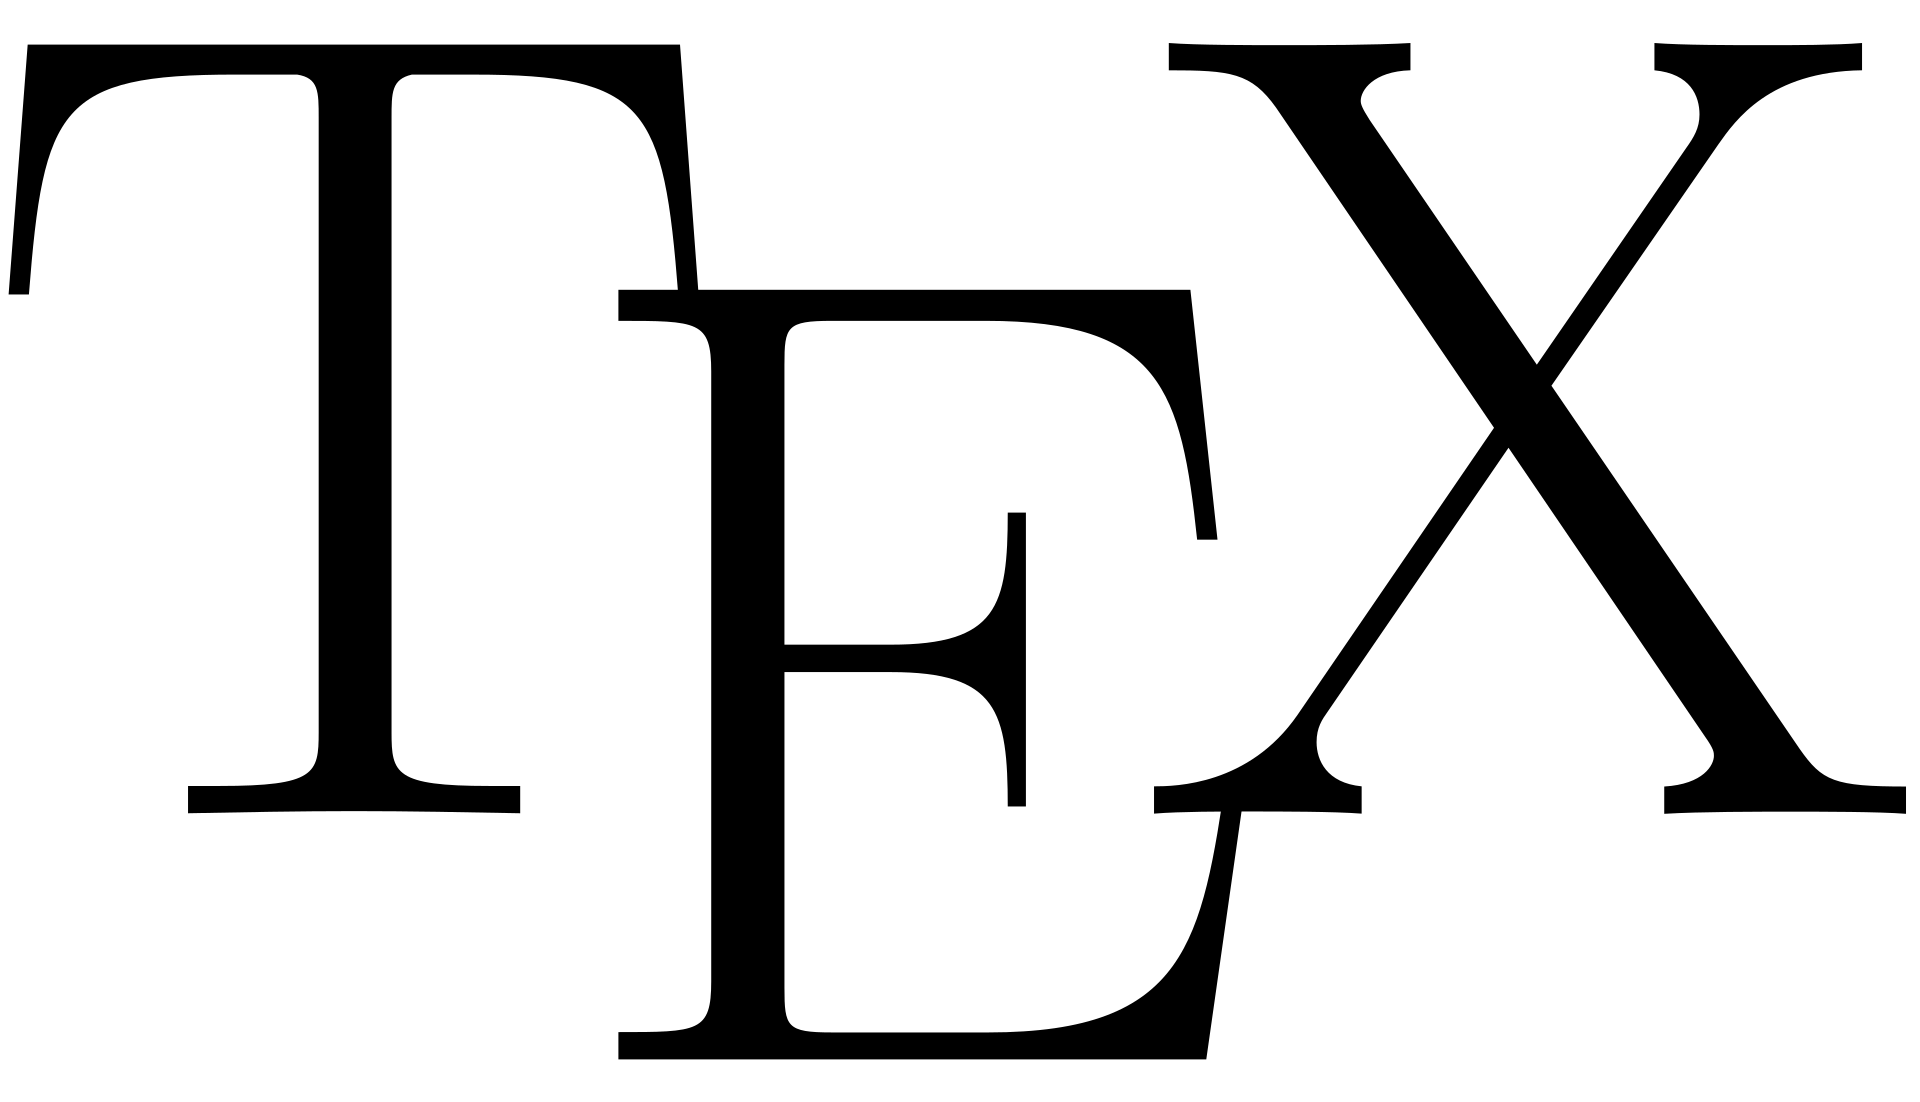
\includegraphics[width=0.7\linewidth]{TeX}
		\caption{Logo de TeX}
		\label{fig:subfig2}
	\end{subfigure}
	\caption{Ejemplo para poner dos figuras juntas. Y citarlas por separado a (\subref{fig:subfig1}) y (\subref{fig:subfig2}).}
	% OJO: el caption siempre va antes del label
	\label{fig:subfigs}
\end{figure}



% Para hacer que quede todo en una misma linea, se puede usar minipage
%\begin{minipage}[t]{\textwidth}
	\begin{lstlisting}[caption={Ejemplo de código (usando los estilos de la cátedra, ver las macros para más detalles)},label=code:for]
r e s = r e c u r s o s
i = 0
w hil e ( i < | e v e n t o s |) do
	i f e v e n t o s [ i ] then
		r e s = ( r e s * apue s t a . c ) * pago . c
	e l s e
		r e s = ( r e s * apue s t a . s ) * pago . s
	e n d i f
	i = i + 1
endwhile
	\end{lstlisting}
%\end{minipage}

Si se pone un label al \verb|lstlisting|, se puede referenciar: Código \ref{code:for}.


\subsection{Macros de la cátedra para especificar}

\begin{proc}{nombre}{\In paramIn : \nat, \Inout paramInout : \TLista{\ent}}{tipoRes}
	%    \modifica{parametro1, parametro2,..}
	\requiere{expresionBooleana1}
	\asegura{expresionBooleana2}
	\aux{auxiliar1}{parametros}{tipoRes}{expresion}
	\pred{pred1}{parametros}{expresion} 
\end{proc}

\aux{auxiliarSuelto}{parametros}{tipoRes}{expresion}
% \paraTodo{variable}{tipo}{expresion}
% \existe{variable}{tipo}{expresion}
% Pueden tener [unalinea] para que no se divida en varias lineas
\pred{predSuelto}{parametros}{\paraTodo[unalinea]{variable}{tipo}{algo \implicaLuego expresion}}
\pred{predSuelto}{parametros}{\existe[unalinea]{variable}{tipo}{algo \yLuego expresion}}



\end{document}
